%----------- slide --------------------------------------------------%
\begin{frame}
\frametitle{ccast LW std}

\begin{center}
  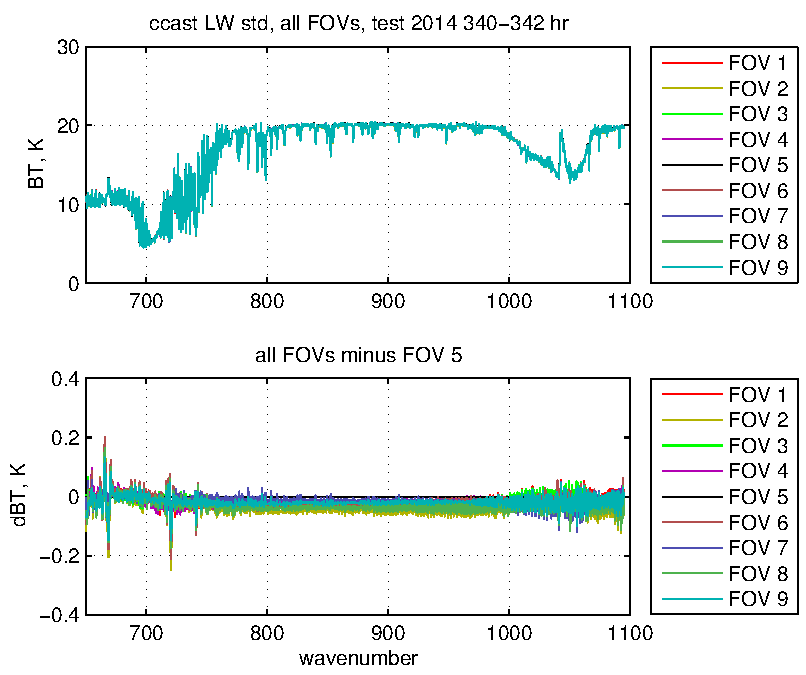
\includegraphics[scale=0.7]{figures/ccast_LW_std_2014_340-342_hr.pdf}
\end{center}

\end{frame}
%----------- slide --------------------------------------------------%
\begin{frame}
\frametitle{noaa LW std}

\begin{center}
  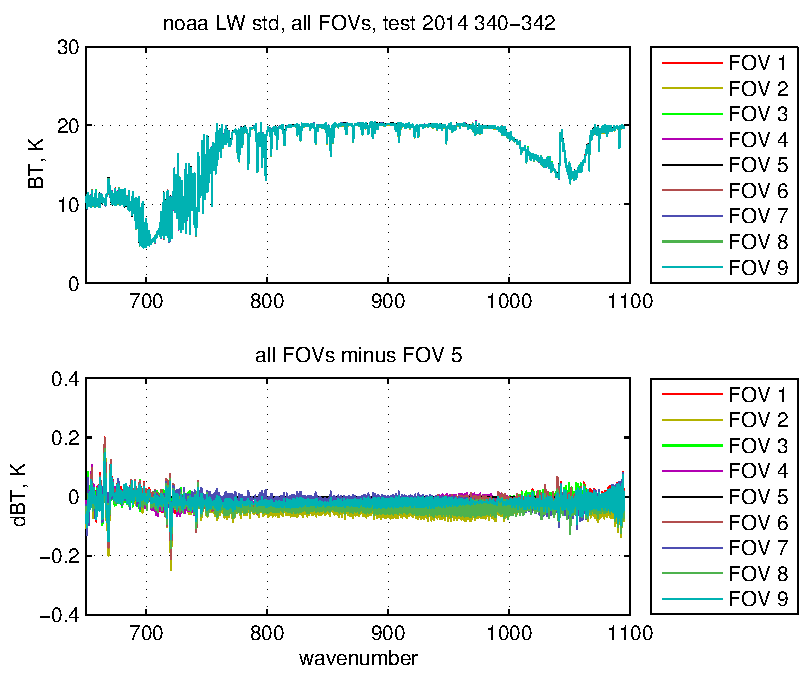
\includegraphics[scale=0.7]{figures/noaa_LW_std_2014_340-342.pdf}
\end{center}

\end{frame}
%----------- slide --------------------------------------------------%
\begin{frame}
\frametitle{ccast MW std}

\begin{center}
  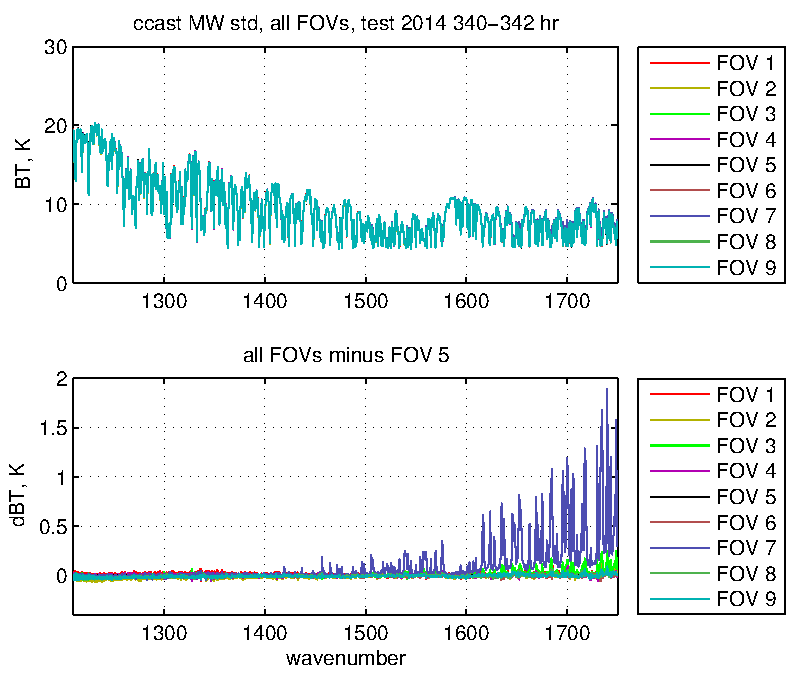
\includegraphics[scale=0.7]{figures/ccast_MW_std_2014_340-342_hr.pdf}
\end{center}

\end{frame}
%----------- slide --------------------------------------------------%
\begin{frame}
\frametitle{noaa MW std}

\begin{center}
  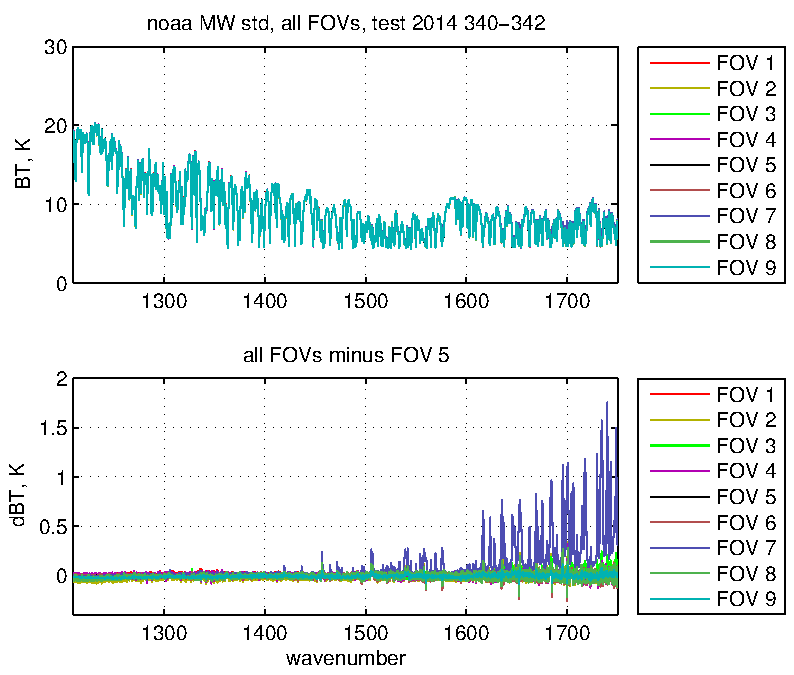
\includegraphics[scale=0.7]{figures/noaa_MW_std_2014_340-342.pdf}
\end{center}

\end{frame}
%----------- slide --------------------------------------------------%
\begin{frame}
\frametitle{ccast SW std}

\begin{center}
  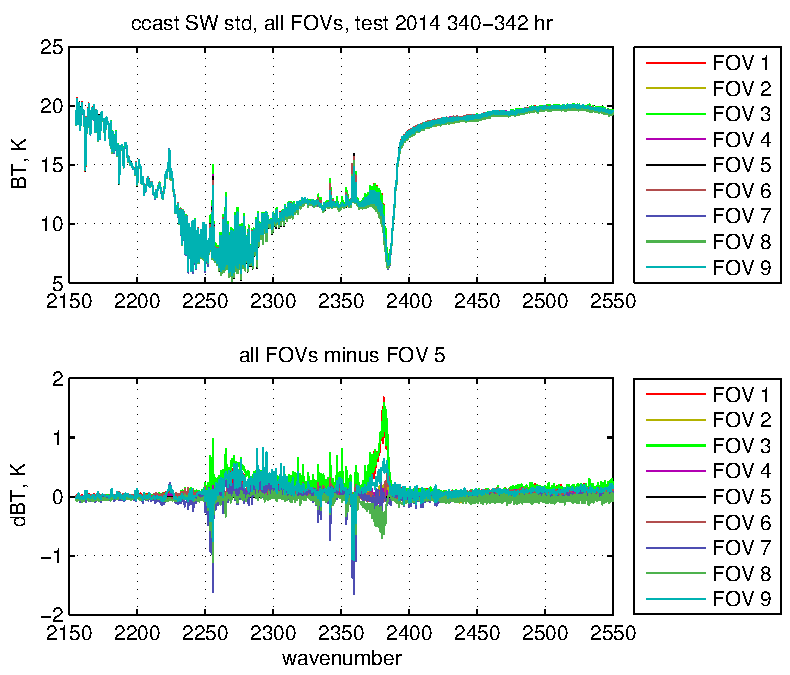
\includegraphics[scale=0.7]{figures/ccast_SW_std_2014_340-342_hr.pdf}
\end{center}

\end{frame}
%----------- slide --------------------------------------------------%
\begin{frame}
\frametitle{noaa SW std}

\begin{center}
  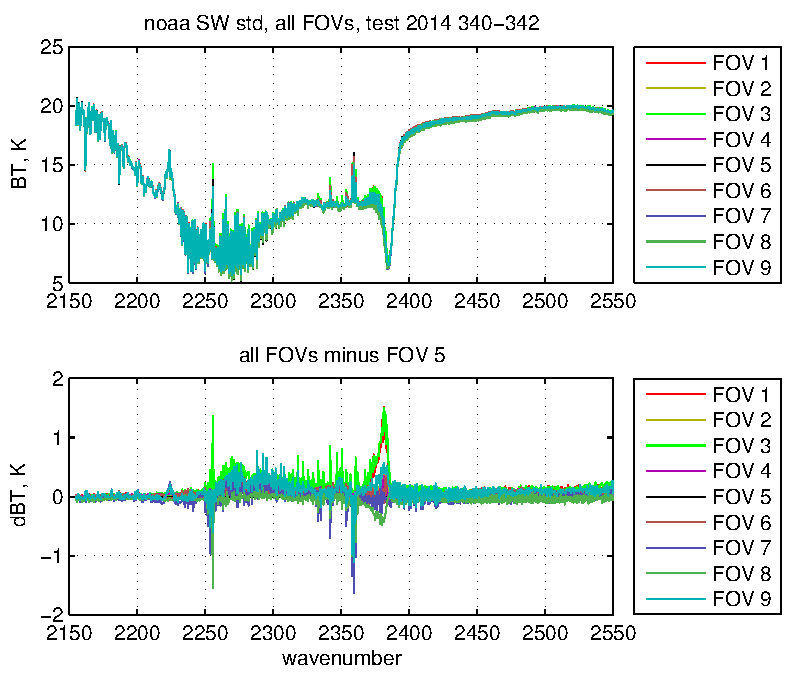
\includegraphics[scale=0.7]{figures/noaa_SW_std_2014_340-342.pdf}
\end{center}

\end{frame}
%----------- slide --------------------------------------------------%
\begin{frame}
\frametitle{calibration equation}

The \ccast\ reference calibration equation is

\[r_{\mbox{\tiny OBS}} = F \cdot r_{\mbox{\tiny ICT}}\cdot f \cdot
  \SA^{-1}\cdot f \cdot \frac{\ES - \SP}{\IT - \SP} \]

\begin{itemize}
  \item $r_{\mbox{\tiny OBS}}$ is calibrated radiance at the user grid
  \item $F$ is Fourier interpolation from sensor to user grid
  \item $f$ is a raised-cosine bandpass filter
  \item $r_{\mbox{\tiny ICT}}$ is expected ICT radiance at the sensor grid
  \item $\SA^{-1}$ is the inverse of the ILS matrix
  \item $\ES$ is earth-scene count spectra
  \item $\IT$ is calibration target count spectra
  \item $\SP$ is space-look count spectra
\end{itemize}

\end{frame}
%----------- slide --------------------------------------------------%
\begin{frame}
\frametitle{calibration notes}

\begin{itemize}

  \item the $\IT$ and $\SP$ looks are averaged over several scans

  \item the UW nonlinearity correction is applied to count spectra
    before application of the calibration equation

  \item as part of the nonlinearity correction we divide the count
    spectra by the numeric filter at the sensor grid, but note this
    cancels out in the ratio $(\ES - \SP) / (\IT - \SP)$

  \item the passband for $f$ is the user grid.  The wings are
    parameters currently set at 15, 20, and 22 \wnum\ for the LW,
    MW, and SW bands

  \item $f \cdot \SA^{-1} \cdot f$ can be considered as a
    physically-based smoothing of the rows and columns of $\SA^{-1}$

  \item $F$ is a zero-filled double Fourier interpolation

\end{itemize}

\end{frame}
%----------- slide --------------------------------------------------%
\begin{frame}
\frametitle{ccast ILS}

the \cris\ \ils\ for $\fov_i$ can be represented as

\[\int_{\mbox{\tiny FOV}_i} \!\!\!\! w_i(\theta)\, \psinc(2 \pi
                 d(v - v_0 \cos \theta ))\, d\theta \]

% f_{v_0}(v) = 
% \int_{\mbox{\tiny FOV}_i}
% \int_{a_i}^{b_i}

\begin{itemize}
  \item $d$ is max \opd
  \item $v$ is frequency
  \item $v_0$ is reference or channel frequency
  \item $\psinc(x) = sin(x)/(n \sin(x/n))$ for $x \ne 0$,  $1$ for
    $x = 0$, where $n$ is the number of points in the sensor grid
   \item $\psinc(2 \pi d(v - v_0 \cos \theta ))$ gives the ILS for a
    single ray at off-axis angle $\theta$
  \item integration is over the intersection of on-axis arcs with
    $\fov_i$, with $w_i(\theta)$ the length of an intersecting arc
    at off-axis angle $\theta$
\end{itemize}

\end{frame}
